\section{Konzeptzeichnungen und Storyboards}

% Bilder sind wichtig für den ersten Eindruck. Vor allem im GDD sind
% Konzeptzeichnungen und Skizzen gut aufgehoben. Auf diese Weise kann man nicht
% nur sich selbst schnell eine Vorstellung von den Ideen machen, sondern auch
% anderen vermitteln, worum es im Spiel geht und wie das Spiel und seine
% Geschichte aussieht.

\missingSection{Konzeptzeichnungen und Storyboards}
\begin{figure}[ht]
	\centering
	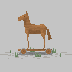
\includegraphics[]{pferd.png}
	\caption{Trojaner}
	\label{fig:pferd}
\end{figure}